\section{Related Work}
\todo[inline]{Describe related work section in FINAL THESIS QUALITY (WORK IN PROGRESS).}

\subsection{RQ1: Constructing the Entity Network}
\todo[inline]{ Entity deduplication. Describe deterministic methods for deduplication. Describe entity linking using edit/Levenshtein distance measures. }
\subsection{RQ2: Process mining insolvency case data}
\todo[inline]{ Describe Wil van Aalst - Process Mining - Play in. Describe methods using log files to deduce the process model.} 
\subsection{RQ3: Text mining unstructured PDF files}
\todo[inline]{ Describe text mining techniques. }
\subsection{RQ4: IS Evaluation by involved parties}
\todo[inline]{ Describe evaluation measures for information systems. }
Shannon and Weaver \cite{shannon_weaver} state that output of an IS can be defined at different levels
\begin{enumerate}
\item \textbf{technical level}: the accuracy and efficiency of the system.
\item \textbf{semantic level}: the success of information conveying the intended meaning.
\item \textbf{effectiveness level}: the effect of information on the receiver 
\end{enumerate}

This implies that factors contributing to a successful IS can also be defined at different levels. DeLone and McLean\cite{delone_mclean:1, delone_mclean:2} have gathered many factors from literature and grouped them into six distinct but interdependent categories, see figure \ref{fig:success_model} below.

\begin{figure}[h]
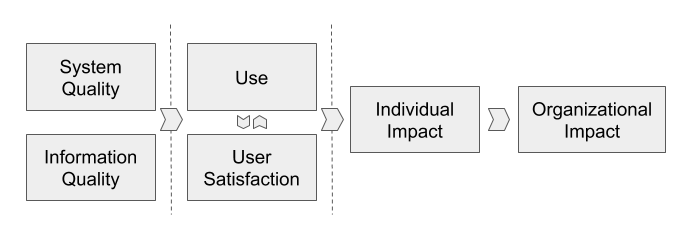
\includegraphics[width=1\linewidth]{images/dm_is_success_model.png}
\caption{DeLone and McLean Information Success Model.}
\label{fig:success_model}
\end{figure}

Each category or aspect of the I/S success measures still contains variables that contribute to success:

\begin{itemize}
\item \textbf{System Quality}: measures the IS itself on the technical level. Example variables are data currency, completeness, and ease of use.
\item \textbf{Information Quality}: measures the IS output such as reports at the semantic level. Example variables are accuracy, precision and relevance.
\item \textbf{Information Use}: measures the actual use of the IS which is where the effectiveness level starts.
\item \textbf{User Satisfaction}: measures satisfaction from the perspective of the user, usually on an interval scale. This category is the mostly used as a single success measure and is fairly subjective.
\item \textbf{Individual Impact}: measures the information effect on the behaviour of the recipient.
\item \textbf{Organizational Impact}: measures the information effect on the performance of the organization.
\end{itemize}
